\section{Level Curves, Graphs, and Surfaces}
\begin{enumerate}
    \item \textbf{Level Curve and Level Surface} \\
    The set of points in the plane where a function $f(x, y)$ has a constant value, i.e. where $f(x, y) = c$
    is called a \textbf{level curve} of $f$. In essence, the set of all points $(x, y, z) \in \R^3$, where
    a function of the \textit{independent} variables has a constant value $z = f(x, y) = c$ is called the
    \textbf{level surface} of $f$.

    \item \textbf{Graph or Surface} \\
    The set of all points $(x, y, f(x, y)) \in \R^3$ for $(x, y)$ in the domain of $f$ is called the
    \textbf{graph} or \textbf{surface} of $f$.

    \item \textbf{Contour Curve} \\
    A plane $z = c$ cuts the surface $z = f(x, y)$ in the points given by $f(x, y) = c$. This curve in space
    is called the \textbf{contour curve} $f(x, y) = c$. The contour curve is a curve in the plane $z = c$,
    whereas the level curve is a curve in the $xy$-plane.
\end{enumerate}

\textbf{Reference Link:}
\reference{https://www.youtube.com/watch?v=acdX4YamDtU}{Visualizing Multi-variable Functions with Contour Plots}

\begin{figure}[h]
    \begin{subfigure}[b]{0.5\textwidth}
        \centering
        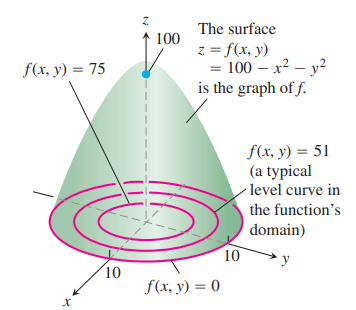
\includegraphics[scale=0.85]{level-curve-1.png}
        \caption{Level Curves}
    \end{subfigure}
    \hfill
    \begin{subfigure}[b]{0.5\textwidth}
        \centering
        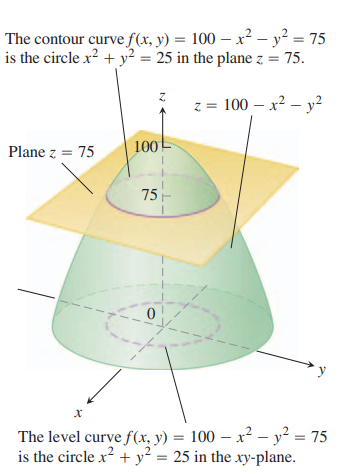
\includegraphics[scale=0.75]{contour-curve-1.png}
        \caption{Contour Curves}
    \end{subfigure}
\end{figure}

\begin{example}
    \normalfont For the plane $z = 50$ on the surface of $z = 75 - x^2 - y^2$:
    \begin{enumerate}
        \item The contour curve is the circle $x^2 + y^2 = 25$ in the plane $z = 50$.
        \item The level curve is $f(x, y) = 75 - x^2 - y^2 = 50$, i.e. the circle $x^2 + y^2 = 25$ in the $xy$-plane.
    \end{enumerate}
\end{example}